\documentclass[12pt]{article}

%\usepackage[margin=1in]{geometry}
\usepackage{amssymb}
\usepackage{amsthm}
\renewcommand\qedsymbol{$\blacksquare$}
\usepackage{multicol}
\usepackage{graphicx}
\graphicspath{ {images/} }
\usepackage{verbatim}

\setlength\parindent{0pt}

\title{\textbf{\Large{Tree Traversal}}}
\author{Ben Gunning}
\date{\today}

\newtheorem{theorem}{Theorem}[section]
\newtheorem{postulate}{Postulate}[section]
\theoremstyle{definition}
\newtheorem{definition}[theorem]{Definition}
\theoremstyle{remark}
\newtheorem{remark}[theorem]{Remark}

\begin{document}
\maketitle

\section*{Abstract}

\section{Introduction}
Tree traversal is a topic that is particularly useful in computer science. In particular, tree traversal is useful for search algorithms, as it helps to characterize the positions of nodes in a tree. This enables a search algorithm, a binary search in particular, to perform an efficient search.

In order to understand the intuition behind tree traversal, it is first necessary to lay some foundation. The definition of a tree is an ample place to start.

\begin{definition}[Tree]
A tree is a finite set of nodes and 1-directional edges (think rays, arrows pointing from one node to another node that can only be followed in one direction) satisfying several conditions.
	\begin{enumerate}
		\item{There does not exist a circuit of nodes. This means that for any node, there is no path of edges that starts from that node and ends at the same node.}
		\item{No two edges are directed at the same node. More formally, no node has multiple parents.}
		\item{The set is connected. In other words, if you allow edges to be traversed both ways, there exists a path between any two nodes.}
	\end{enumerate}
\end{definition}

A couple of definitions make naming and reference to certain nodes and relationships between nodes easier and more intuitive.

\begin{definition}
A node is a \emph{parent} of another node if there is an edge from the former to the latter. The latter node would be said to be a \emph{child} of the former node. The set of all children of the children of ... of a node is the set of that node's \emph{descendents}. Similarly, the set containing a node's parent,
the parent's parent, and so on (to the root) is called that node's \emph{ancestors}.
\end{definition}

Next we should define a root, an aspect of a tree. We will also need to prove some characteristics such as the existence and uniqueness of roots.

\begin{definition}[Root]
A root is a node in a tree that has no parents. Alternatively, a root is a node to which no edges point.
\end{definition}

\begin{postulate}[Existence of Roots]
Every tree has a root.
\end{postulate}

\begin{proof}
We proceed with a proof by contradiction. Consider a tree with no root. Since we've defined trees to be necessarily finite, we may label nodes as $1 , 2 , ... , n$. Start with node $n$ and consider its parent. There are $n-1$ possible parents for node $n$. Without loss of generality, suppose that
$n-1$ is the parent of $n$. Next consider node $n-1$. It has $n-2$ possible parents, since $n$ cannot be a parent to $n-1$ without violating the first property of trees. Without loss of generality, let $n-2$ be the parent of $n-1$. We may use the procedure, noting that no previously considered nodes
could be a parent to a newly considered node without violating the first property, until we have considered all but one nodes. Without loss of generality, let the last node be $1$. There are no possible parents for node $1$ that do not violate the first property of trees. Hence, $1$ has no parents, and
we have a contradiction.
\end{proof}

\begin{postulate}[Uniqueness of Roots]
Every tree has no more than one root.
\end{postulate}

\begin{proof}
Consider a tree of $n$-many nodes ($1$ through $n$). Let nodes $1$ and $2$ be two roots of our tree. Since $1$ and $2$ are two nodes, by the third property, there is a path (ignoring orientation) between $1$ and $2$. We have three possible cases to consider for this path.
\begin{itemize}
	\item{All of the edges in the path from $1$ to $2$ form a chain (observing orientation) from $1$ to $2$. This contradicts our claim that $2$ is a root.}
	\item{All of the edges in the path from $1$ to $2$ form a chain (observing orientation) from $2$ to $1$. This contradicts our claim that $1$ is a root.}
	\item{Two edges in the path from $1$ to $2$ point to the same node. This contradicts the second property.}
\end{itemize}
These cases are exhaustive, and each leads to a contradiction. Hence, the assumption must be false.
\end{proof}

These two postulates prove that every tree has exactly one root (using our aforementioned definition). In contrast, there is no limit on the number of nodes of the next type in a given tree.

\begin{definition}[Leaf]
A leaf is a node that is the parent to no other nodes.
\end{definition}.

By the same logic as our previous existence proof, it is easy to prove the following result.

\begin{postulate}
Every tree has a leaf.
\end{postulate}

With this foundation on trees in mind, we will now introduce a type of tree that is particularly interesting for the development of search algorithms.

\begin{definition}[Binary Tree]
A binary tree is a tree in which every node is the parent of no more than two child nodes.
\end{definition}

Binary trees are useful for the purpose of binary search algorithms. However, for these purposes, there is a logical question that follows: How can we characterize a binary tree more simply?

\section{Characterization}
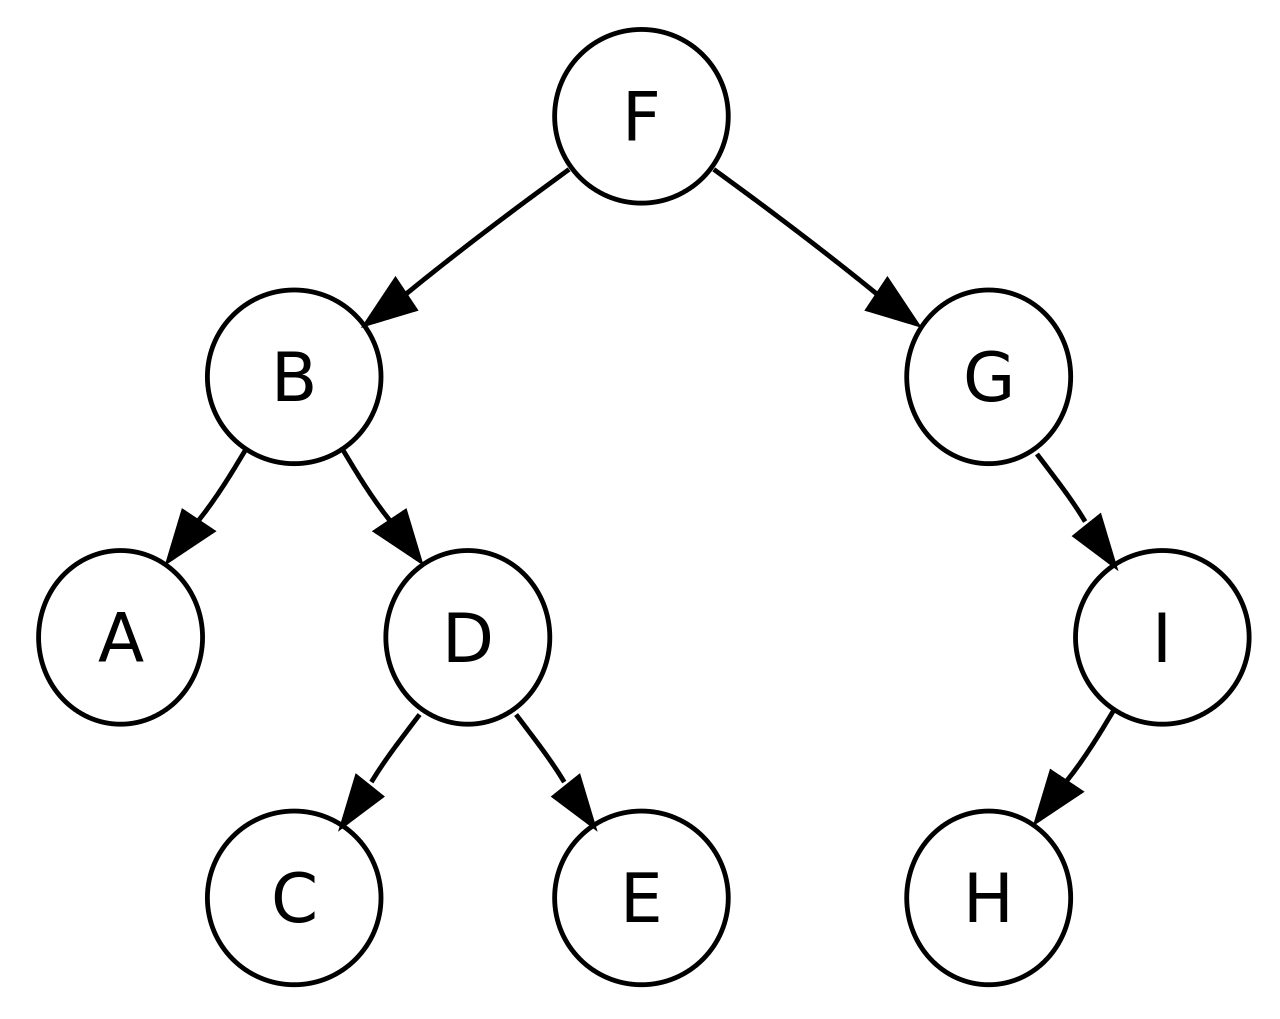
\includegraphics[scale=.125]{Binary}

Consider the binary tree above. How can we represent an arbitrary binary tree such as this by means of an ordered list of nodes? In order to do this, we will rely on recursively deconstructing our trees into smaller \emph{subtrees}.

\begin{definition}
Given a node within a binary tree, we may define its children (if any) by the terminology left child and right child, assigned to children based on a general direction that is consistent across all references to the tree. The tree formed by the left child and all of its descendents is called the \emph{left subtree} of the original
node. Similarly, the tree formed by the right child and all of its descendents is called the \emph{right subtree} of the original node.
\end{definition}

Note that the root, the root's left subtree, and the root's right subtree provide the foundation upon which we may construct a recursive method of ordering the nodes of a binary tree. We shall now define several such methods of ordering the nodes of a binary tree.

\begin{definition}[Pre-Order Traversal]
Given a binary tree, we can perform what is called a \emph{pre-order traversal} of the tree by applying a recursive operation (beginning with the root) in the following manner:
\begin{enumerate}
	\item{Display the node}
	\item{Recursively perform this operation on the node's left subtree}
	\item{Recursively perform this operation on the node's right subtree}
\end{enumerate}
\end{definition}

\begin{definition}[In-Order Traversal]
Given a binary tree, we can perform what is called an \emph{in-order traversal} of the tree by applying a recursive operation (beginning with the root) in the following manner:
\begin{enumerate}
	\item{Recursively perform this operation on the node's left subtree}
	\item{Display the node}
	\item{Recursively perform this operation on the node's right subtree}
\end{enumerate}
\end{definition}

\begin{definition}[Post-Order Traversal]
Given a binary tree, we can perform what is called a \emph{post-order traversal} of the tree by applying a recursive operation (beginning with the root) in the following manner:
\begin{enumerate}
	\item{Recursively perform this operation on the node's left subtree}
	\item{Recursively perform this operation on the node's right subtree}
	\item{Display the node}
\end{enumerate}
\end{definition}

\end{document}